\chapter{ GANTT PRÉVISIONNEL}

Le diagramme de Gantt est un outil de planification très utile voire même indispensable dans la gestion d'un projet informatique. Il permet de visualiser les différentes tâches d'un projet et leur niveau d'avancement ce qui améliore considérablement l'organisation et la gestion du temps disponible pour respecter les délais fixés pour la livraison d'un produit final au client. C'est donc tout naturellement, après la réception du sujet et nos divers échanges avec le client qu'on a établi le diagramme prévisionnel ci-dessous. Ce diagramme tient donc étroitement compte de notre compréhension initiale du sujet et des tâches indispensables identifiées pour le réaliser. 

\begin{figure}[H]
    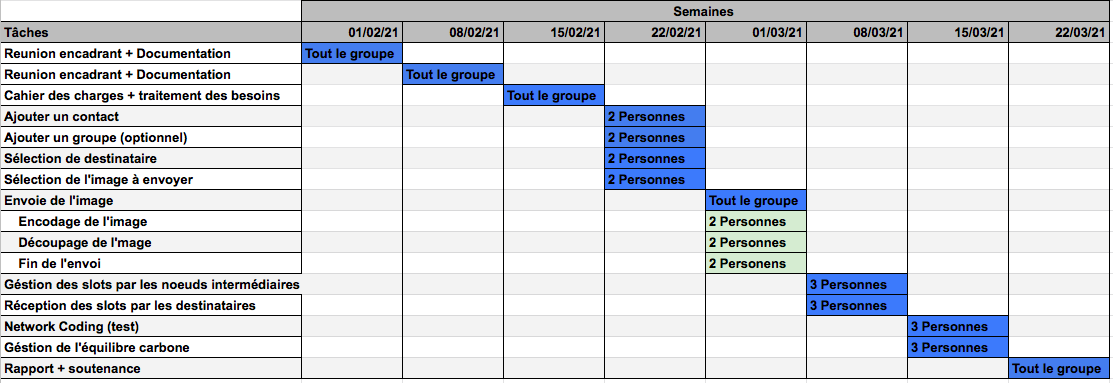
\includegraphics[width=18cm]{images/gantt.png}
    \caption{Gantt prévisionnel.}
\end{figure}

Très vite, après le début du projet, lors de nos rencontres hebdomadaires avec le client et les autres groupes impliqués dans ce projet, nous nous sommes rendus compte que les tâches succinctes qu'on avait identifiées au préalable seront amenées à évoluer/changer. C'est donc naturellement au fur des semaines qu'on a amélioré notre diagramme pour le mettre en adéquation avec l'avancement du projet. 

\begin{figure}[H]
    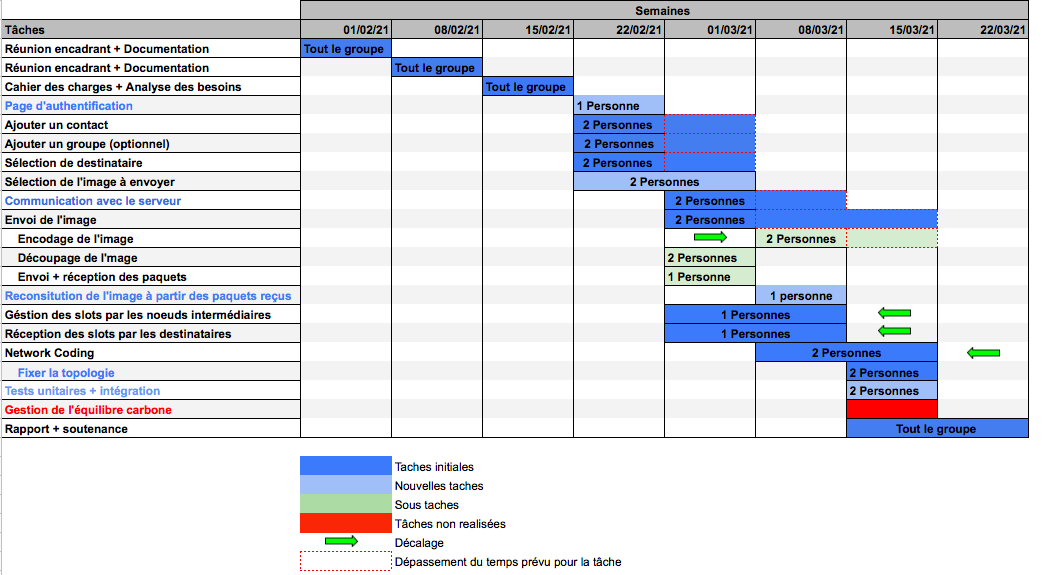
\includegraphics[width=18.5cm]{images/gantbis.png}
    \caption{Gantt effectif.}
\end{figure}

Identifier les tâches à effectuer est une chose relativement accessible, mais quantifier le temps de travail nécessaire pour la réalisation de certaines tâches demande de l'expérience dans la réalisation de ces dernières. Nous avons réussi à respecter les délais prévus durant le premier mois, mais on a dû adapter beaucoup de tâches dans la réalisation de la seconde partie du projet. 



